% !TEX TS-program = pdflatex
% !TEX encoding = UTF-8 Unicode

% This is a simple template for a LaTeX document using the "article" class.
% See "book", "report", "letter" for other types of document.

\documentclass[11pt]{article} % use larger type; default would be 10pt

\usepackage[utf8]{inputenc} % set input encoding (not needed with XeLaTeX)

%%% Examples of Article customizations
% These packages are optional, depending whether you want the features they provide.
% See the LaTeX Companion or other references for full information.

%%% PAGE DIMENSIONS
\usepackage{geometry} % to change the page dimensions
% \geometry{letterpaper} % or letterpaper (US) or a5paper or....
% \geometry{margin=2in} % for example, change the margins to 2 inches all round
% \geometry{landscape} % set up the page for landscape
%   read geometry.pdf for detailed page layout information

\usepackage{graphicx} % support the \includegraphics command and options

% \usepackage[parfill]{parskip} % Activate to begin paragraphs with an empty line rather than an indent

%%% PACKAGES
\usepackage{booktabs} % for much better looking tables
\usepackage{array} % for better arrays (eg matrices) in maths
\usepackage{paralist} % very flexible & customisable lists (eg. enumerate/itemize, etc.)
\usepackage{verbatim} % adds environment for commenting out blocks of text & for better verbatim
\usepackage{subfig} % make it possible to include more than one captioned figure/table in a single float
% These packages are all incorporated in the memoir class to one degree or another...

%%% HEADERS & FOOTERS
\usepackage{fancyhdr} % This should be set AFTER setting up the page geometry
\pagestyle{fancy} % options: empty , plain , fancy
\renewcommand{\headrulewidth}{0pt} % customise the layout...
\lhead{}\chead{}\rhead{}
\lfoot{}\cfoot{\thepage}\rfoot{}

%%% SECTION TITLE APPEARANCE
\usepackage{sectsty}
\allsectionsfont{\sffamily\mdseries\upshape} % (See the fntguide.pdf for font help)
% (This matches ConTeXt defaults)

%%% ToC (table of contents) APPEARANCE
\usepackage[nottoc,notlof,notlot]{tocbibind} % Put the bibliography in the ToC
\usepackage[titles,subfigure]{tocloft} % Alter the style of the Table of Contents
\renewcommand{\cftsecfont}{\rmfamily\mdseries\upshape}
\renewcommand{\cftsecpagefont}{\rmfamily\mdseries\upshape} % No bold!

%%% END Article customizations

%%% The "real" document content comes below...

\title{Project 2 - Genetic Programming}
\author{Tao Zhang}
\date{March 26th, 2014} % Activate to display a given date or no date (if empty),
         % otherwise the current date is printed 

\begin{document}
\maketitle

\section{Abstract}

\begin{tabular}{|l|p{4in}|}
\hline
Algorithm &  Steady-state\\
\hline
Population size & 100\\
\hline
Selection method & Tournament\\
\hline
Crossover method & Swap two random subtrees in two parents\\ 
\hline
Crossover rate & 90\% Non-terminal, 10\% Terminal\\
\hline
Mutation method & Change the type of one random subnode\\
\hline
Operator/non-terminal set & ${+, -, *, /}$\\
\hline
Terminal set & 0-9, x\\
\hline
Fitness function & $\surd \sum e^2_i$\\
\hline
Size control (if any) & \\
\hline
\end{tabular}


\newpage
Graph showing average and best fitnesses evolving over time. 

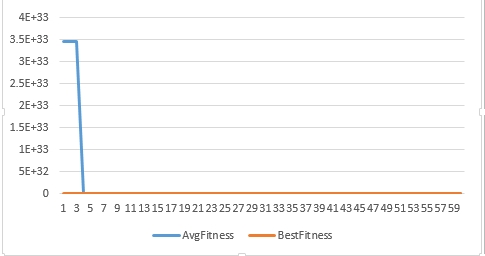
\includegraphics[scale=.7]{First60.jpg}

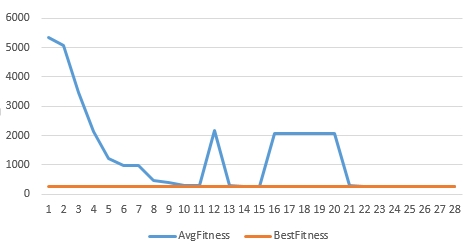
\includegraphics[scale=.7]{60to90.jpg}

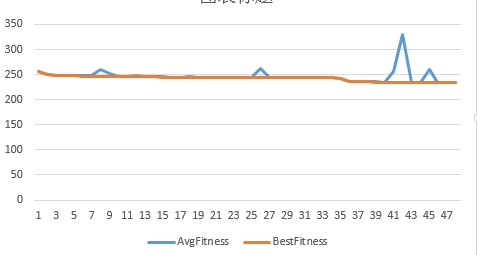
\includegraphics[scale=.7]{90to1000.jpg}


\newpage
Graph showing test points and best evolved function.

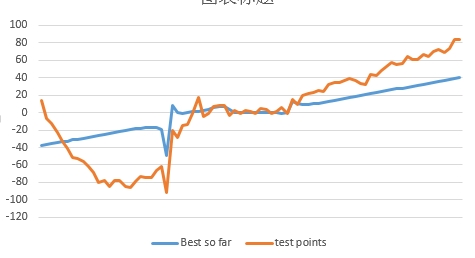
\includegraphics[scale=1]{err.jpg}

\section{Discussion}
\subsection{Average Fitness}
\paragraph{So far, the best fitness and avg fitness is going better and better when the running time goes on. I got the best fitness around 70 during my test. }
\paragraph{As the first graph shown, the average fitness is really high at the very begining, and has a fast drop for first several runs. Then during 60 to 90 running times, the slope becomes small and the fitness still drops a lot. Finally, after 90 running times, the change of fitness is really small. But if I add enough running times, the fitness would be able to be close to 0.}
\paragraph{There are several average fitnesses went very high (changed a lot), which is shown on the second and third graphs. I think that is caused by mutation and crossover, which is unescapable.}

\subsection{Best Fitness}
\paragraph{The best fitness is always less than the average fitness, and really changed a little.}

\subsection{Best Evolved Function}
\paragraph{The graph is looking good I think...}

\subsection{Conclusion}
\paragraph{Overall, my Genetic Programming works fine. I believe if I add more non-terminal sets, and do some size control, my GP would be better.}

\end{document}
